\chapter{Use Case Spécification 1104 - Définir un rendez-vous}

\section{Introduction}

\subsection{Objectifs du document}
Ce document présente aux utilisateurs les spécifications fonctionnelles du \texttt{U.C.},
1104, Définir un rendez-vous, (C, R) afin que le médecin puisse le valider.

\subsection{Domaine de définition du document}
La description du \texttt{U.C.} est complète pour les points 2 à 8. Par contre, le
diagramme d’activités se limite à celui qui présente la création d’un nouveau 
rendez-vous (il faudrait y ajouter la suppression d’un rendez-vous). 

\subsection{Définitions, acronymes et abréviations}
Définition INAMI : voir étude de cas et MCD\footnote{\href{../MCD/MCD.pdf}{voir document M.C.D.}}.

\subsection{Références}
\begin{itemize}
	\item[] Étude de cas de l'agenda
		médical\footnote{\href{../Enonce_Travail_Synthese_14-15.pdf}{voir
		étude de cas}}
	\item[] M.C.D. de \texttt{Medicagenda}\footnote{\href{../MCD/MCD.pdf}{voir document M.C.D.}}
	\item[] M.C.T. de \texttt{Medicagenda}\footnote{\href{./MCT.pdf}{voir document M.C.T.}}
\end{itemize}
\newpage

\section{Définition de Use Case}
\subsection{Identifiant et nom}
\texttt{U.C. 1104} - Définir un rendez-vous (C, R).
\subsection{Brève description}
Ce \texttt{U.C.} permet au médecin ou au patient de définir un rendez-vous.
\subsubsection{Définir un rendez-vous}
Cette définition peut se faire
\begin{itemize}
	\item directement par le médecin,
	\item directement par le patient.
\end{itemize}

La définition implique \texttt{l'enregistrement d'un compte patient} si il n'existe pas.
\newpage

\section{Flux}
\subsection{Flux de base}
Le patient commence par s'identifier sur son compte personnel. 
Si son compte n'existe pas, un message apparaitra pour le prévenir et l'inviter
à le créer. Il y aura, si acceptation, affichage des champs obligatoires à
remplir. Après validation et confirmation, il peut s'identifier auprès de la plateforme.
Le patient va, ensuite, sélectionner le médecin auprès duquel il souhaite
prendre rendez-vous à travers une boite de recherche ou un menu déroulant par
ordre :
\begin{itemize}
	\item alphabétique,
	\item de localisation
	\item ou de spécialité.
\end{itemize}

Si celui-ci n'existe pas, un fenêtre apparaitra permettant d'entrer les données 
de ce dernier pour ensuite traiter, par la plateforme, la
demande d'enregistrement auprès du médecin susdit et le patient retourne sur
son menu principal.
Si il existe, le patient choisira, dans l'agenda du médecin, la date qu'il
souhaite. Si cette date ne contient pas de disponibilité souhaitée, ou de
disponibilité souhaitée libre, le patient recherchera une autre date qui le 
convient.
Une fois la disponibilité sélectionnée, il sera demandé d'entrer un commentaire,
ou non à l'attention du médecin. Un message récapitulatif apparaitra dans une
fenêtre demandant d'accepter la demande et les conditions d'annulation.

\subsection{Flux alternatifs}

\subsubsection{Abandon du U.C.}
A tout moment, le patient peut abandonner l'enregistrement du rendez-vous pour
peu qu'il n'ai pas déjà confirmé.
\newpage

\section{Acteurs, mode, performances, exigences particulières}
\subsection{Acteurs}
Patient ou médecin.
\subsection{Mode}
Interactif unitaire.
\subsection{Événement déclencheur}
Le besoin, d'un patient ou d'un médecin, d'établir un rendez-vous chez un
spécialiste.
Techniquement :
\begin{itemize}
	\item depuis le compte d'un médecin,
	\item depuis le compte d'un patient.
\end{itemize}

\subsection{Performance}
\texttt{Sans Objet}
\subsection{Exigences particulières}
\texttt{Sans Objet}
\newpage

\section{Conditions préalables}
\subsection{Création d'un compte patient}
Pour l'associer à un rendez-vous.
\subsection{Création d'un compte médecin}
Pour créer un agenda public.
\subsection{Définition d'une disponibilité}
Pour permettre au patient de créer un rendez-vous.

\section{Conditions postérieures}
Si abandon du \texttt{U.C.}, le système se retrouve dans l'état où il était avant le
lancement du \texttt{U.C.}.
\newpage

\section{Points d'inclusion et d'extension}
\subsection{Extension}
\texttt{Aucune n'a été déduite de l'analyse}.
\subsection{Inclusion}
\texttt{Aucune n'a été déduite de l'analyse}.
\newpage

\section{Règles de gestion}
\subsection{Classes concernées}
\begin{center}
	\begin{longtable}{|p{2.2cm}|p{2.2cm}|p{2.2cm}|p{2.2cm}|}
		\hline
		 Compte patient & Compte médecin & Disponibilité & Rendez-vous \\
		\hline
		 CR & R & RU & C \\
		\hline
	\end{longtable}
\end{center}
\subsection{Validation des encodages de données}
Les données seront conformes aux formats, aux types et aux contraintes définis
dans le M.C.D. Sinon, affichage d’un message (message standard de l'interface) 
demandant la correction avant sauvegarde des données.
En particulier, validation du numéro INAMI encodé par un organisme externe.

\subsection{Messages}
\begin{itemize}
	\item ``Numéro INAMI en attente de validation''
	\item ``Compte patient non existant dans la base de données''
	\item ``Compte médecin introuvable dans la base de données''
	\item ``Données entrées non valides''
\end{itemize}
\newpage

\section{Diagramme d'activités}
\begin{figure}[hb]
	\centering
	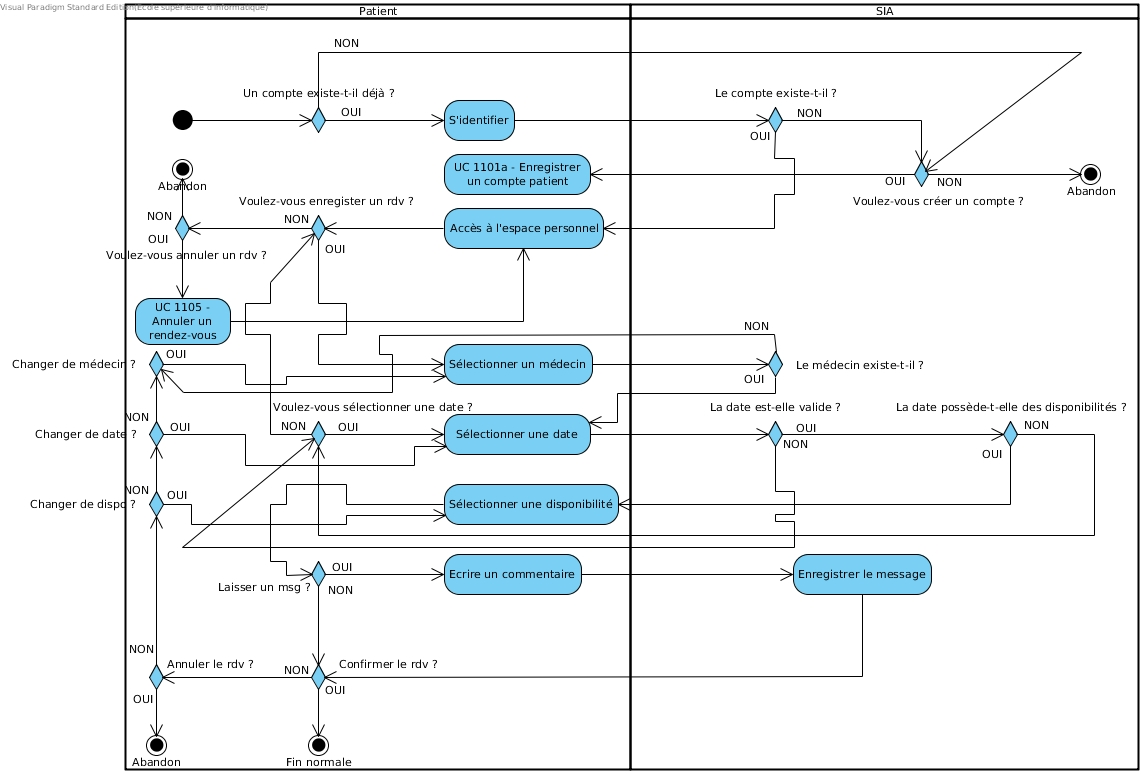
\includegraphics[scale=0.4]{MCT/activiteUC1104.jpg}
	\caption{Diagramme d'activité : \texttt{U.C. 1104}}
	\label{fig:act1104}
\end{figure}
\newpage

\section{Interface utilisateur}
\subsection{Exigences spéciales}
\texttt{S.O.}
\subsection{Aspect}
\begin{figure}[hb]
	\centering
	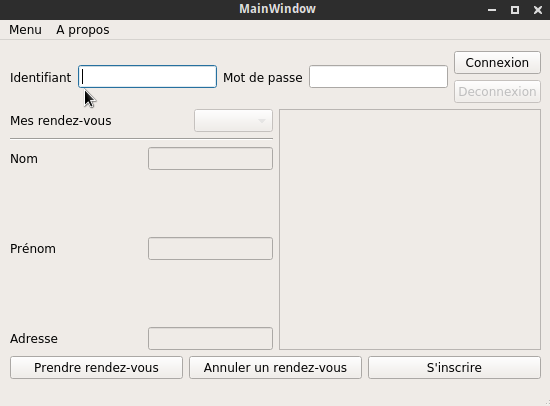
\includegraphics[scale=0.4]{MCT/GUI/workspace.png}
	\caption{Workspace}
	\label{fig:workspace}
\end{figure}
\begin{figure}[hb]
	\centering
	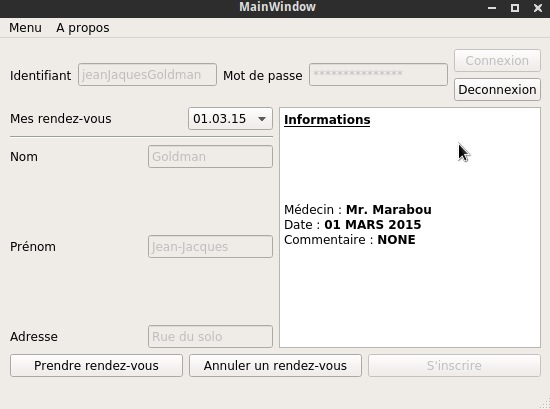
\includegraphics[scale=0.4]{MCT/GUI/connected.png}
	\caption{Workspace connecté}
	\label{fig:wrkconnected}
\end{figure}
\begin{figure}[hb]
	\centering
	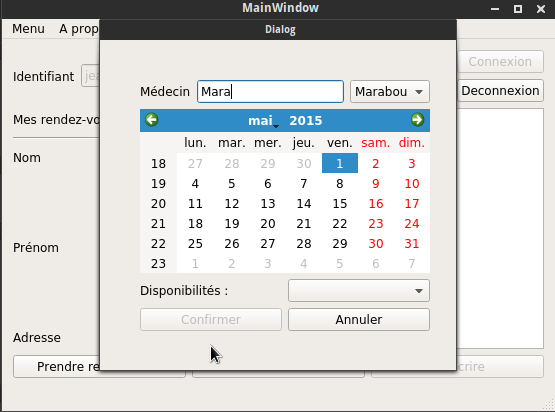
\includegraphics[scale=0.4]{MCT/GUI/rdv.png}
	\caption{Prise de rendez-vous}
	\label{fig:rdv}
\end{figure}
\begin{figure}[hb]
	\centering
	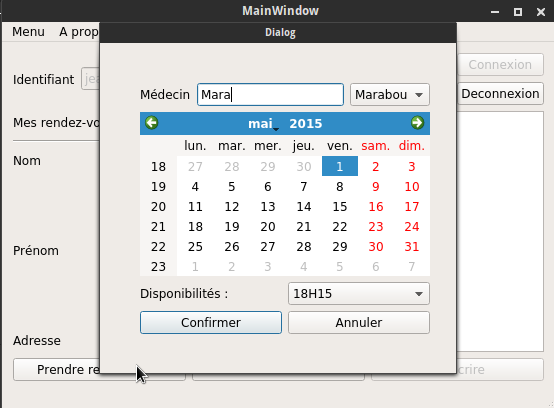
\includegraphics[scale=0.4]{MCT/GUI/rdvConfirm.png}
	\caption{Confirmation de rendez-vous}
	\label{fig:rdvConfirm}
\end{figure}
\newpage
\subsection{Règles de contrôle}
\texttt{Non demandé}

